\documentclass{standalone}
\usepackage{tikz}
\usetikzlibrary{patterns, positioning}
\usepackage[sfdefault]{ClearSans} %% option 'sfdefault' activates Clear Sans as the default text font
\usepackage[T1]{fontenc}

\begin{document}
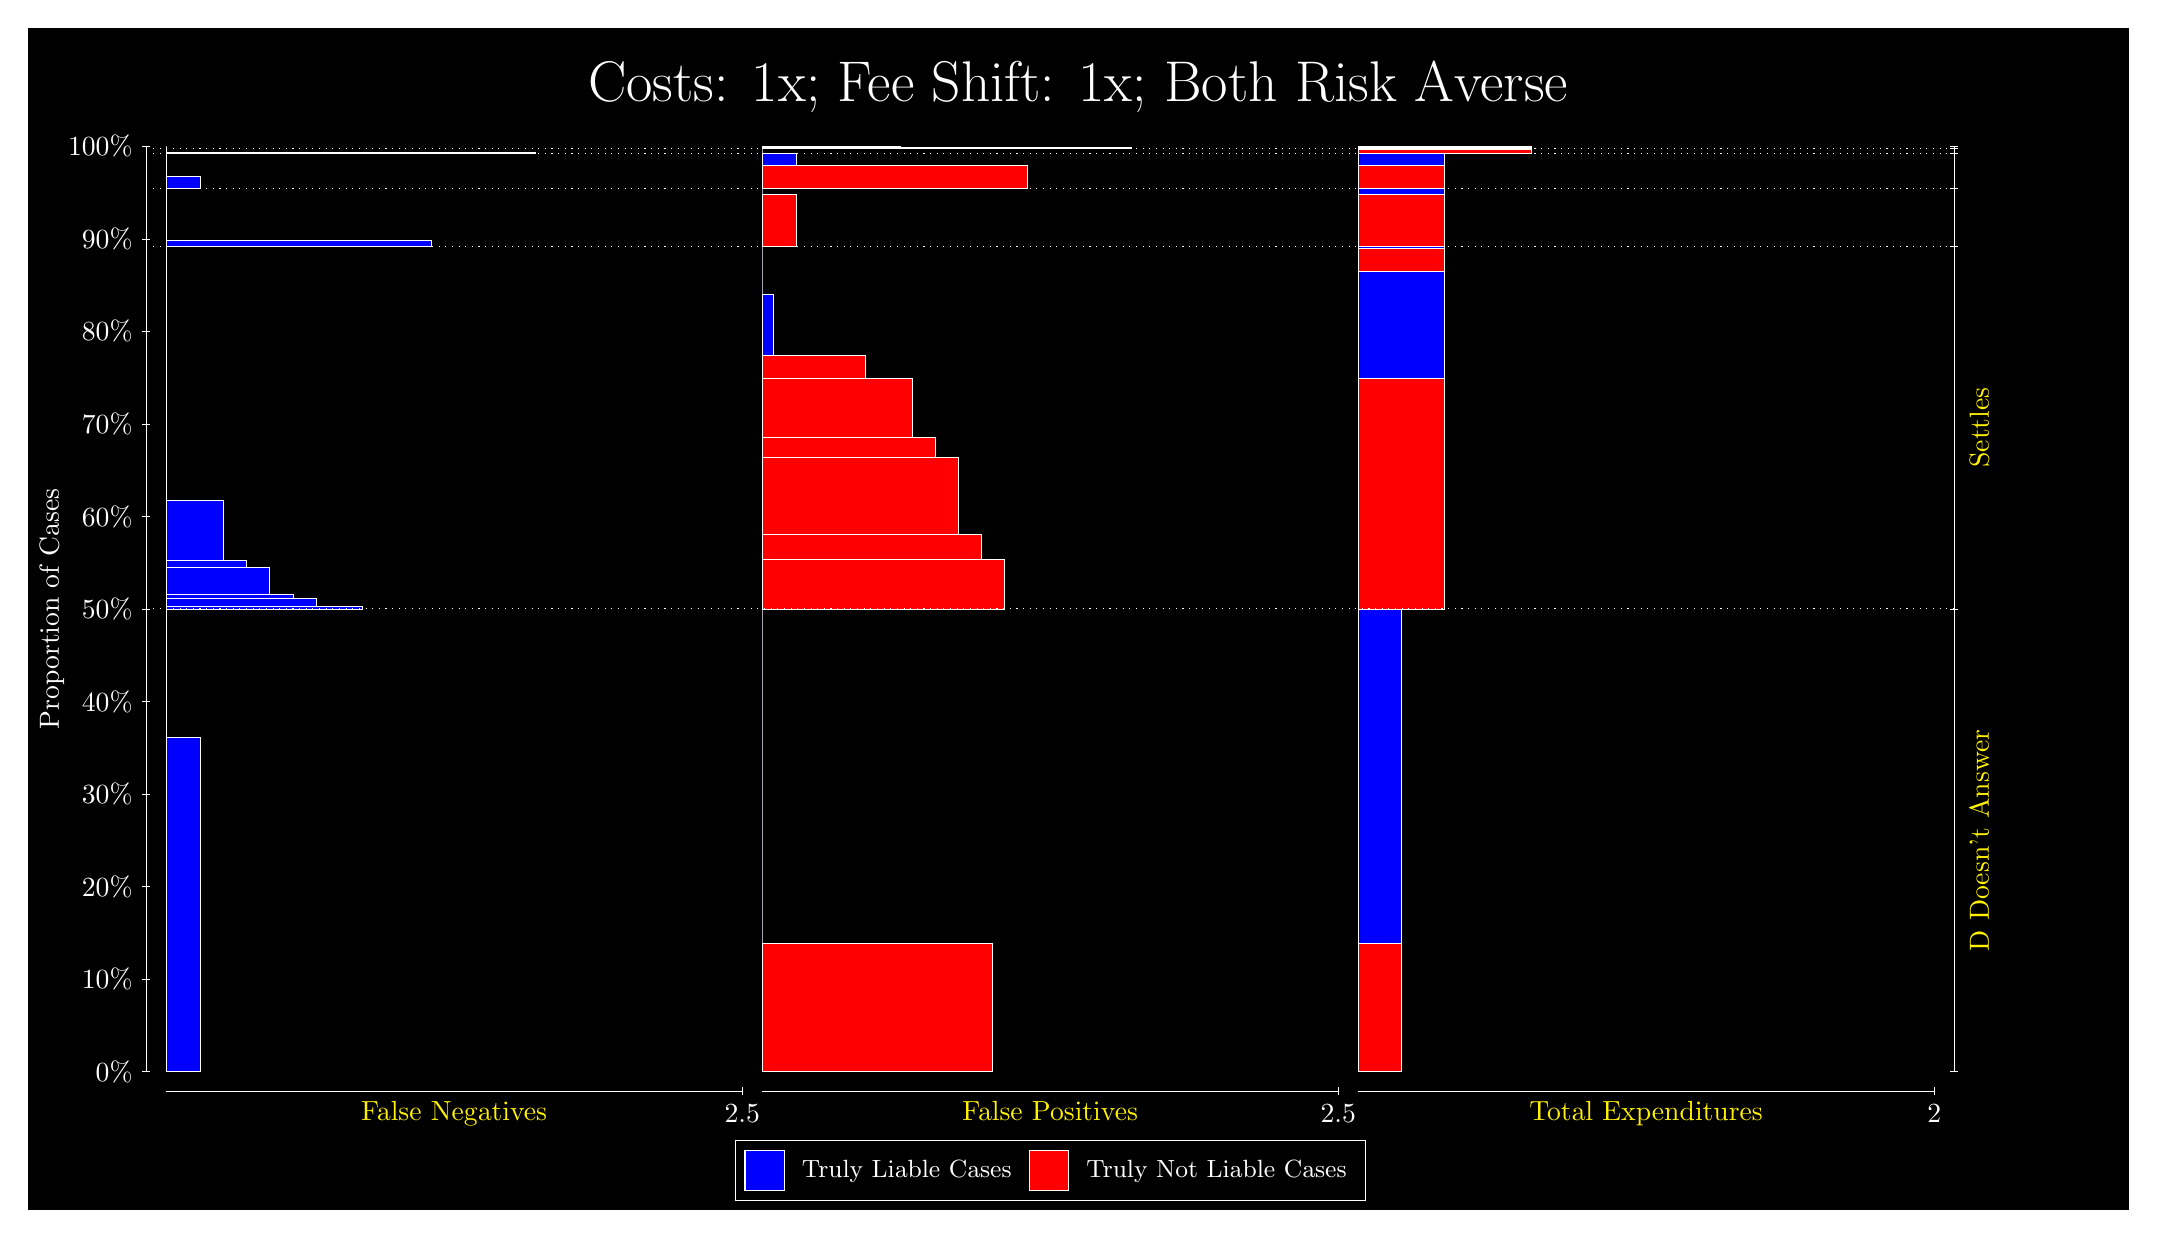
\begin{tikzpicture}
\draw[fill=black] (0,0) rectangle (26.667,15);
\draw[text=white] (0,13.5) rectangle (26.667,15) node[midway] {\huge Costs: 1x; Fee Shift: 1x; Both Risk Averse};
\draw[white, very thin] (1.5,1.75) -- (1.5,13.5);
\node[rotate=90, text=white, anchor=center] at (0.3, 7.625) {Proportion of Cases};
\draw[white, very thin] (1.45,1.75) -- (1.55,1.75);
\node[text=white, anchor=east] at (1.45, 1.75) {0\%};
\draw[white, very thin] (1.45,2.925) -- (1.55,2.925);
\node[text=white, anchor=east] at (1.45, 2.925) {10\%};
\draw[white, very thin] (1.45,4.1) -- (1.55,4.1);
\node[text=white, anchor=east] at (1.45, 4.1) {20\%};
\draw[white, very thin] (1.45,5.275) -- (1.55,5.275);
\node[text=white, anchor=east] at (1.45, 5.275) {30\%};
\draw[white, very thin] (1.45,6.45) -- (1.55,6.45);
\node[text=white, anchor=east] at (1.45, 6.45) {40\%};
\draw[white, very thin] (1.45,7.625) -- (1.55,7.625);
\node[text=white, anchor=east] at (1.45, 7.625) {50\%};
\draw[white, very thin] (1.45,8.8) -- (1.55,8.8);
\node[text=white, anchor=east] at (1.45, 8.8) {60\%};
\draw[white, very thin] (1.45,9.975) -- (1.55,9.975);
\node[text=white, anchor=east] at (1.45, 9.975) {70\%};
\draw[white, very thin] (1.45,11.15) -- (1.55,11.15);
\node[text=white, anchor=east] at (1.45, 11.15) {80\%};
\draw[white, very thin] (1.45,12.325) -- (1.55,12.325);
\node[text=white, anchor=east] at (1.45, 12.325) {90\%};
\draw[white, very thin] (1.45,13.5) -- (1.55,13.5);
\node[text=white, anchor=east] at (1.45, 13.5) {100\%};

\draw[white, very thin] (24.457,1.75) -- (24.457,13.5);
\draw[white, very thin] (24.407,1.75) -- (24.507,1.75);
\node[anchor=west] at (24.407, 1.75) {};
\draw[white, very thin] (24.407,7.6249) -- (24.507,7.6249);
\node[anchor=west] at (24.407, 7.6249) {};
\draw[white, very thin] (24.407,12.232) -- (24.507,12.232);
\node[anchor=west] at (24.407, 12.232) {};
\draw[white, very thin] (24.407,12.966) -- (24.507,12.966);
\node[anchor=west] at (24.407, 12.966) {};
\draw[white, very thin] (24.407,13.407) -- (24.507,13.407);
\node[anchor=west] at (24.407, 13.407) {};
\draw[white, very thin] (24.407,13.478) -- (24.507,13.478);
\node[anchor=west] at (24.407, 13.478) {};
\draw[white, very thin] (24.407,13.5) -- (24.507,13.5);
\node[anchor=west] at (24.407, 13.5) {};

\draw[white, very thin, fill=blue] (1.75,1.75) rectangle (2.1891,5.9985);
\draw[white, very thin, fill=red] (1.75,5.9985) rectangle (1.75,7.6249);
\draw[white, very thin, fill=blue] (1.75,7.6249) rectangle (4.2384,7.6532);
\draw[white, very thin, fill=blue] (1.75,7.6532) rectangle (3.6529,7.755);
\draw[white, very thin, fill=blue] (1.75,7.755) rectangle (3.3602,7.8104);
\draw[white, very thin, fill=blue] (1.75,7.8104) rectangle (3.0674,8.1545);
\draw[white, very thin, fill=blue] (1.75,8.1545) rectangle (2.7746,8.2406);
\draw[white, very thin, fill=blue] (1.75,8.2406) rectangle (2.4819,9.0095);
\draw[white, very thin, fill=red] (1.75,9.0095) rectangle (1.75,12.232);
\draw[white, very thin, fill=blue] (1.75,12.232) rectangle (5.1167,12.303);
\draw[white, very thin, fill=red] (1.75,12.303) rectangle (1.75,12.966);
\draw[white, very thin, fill=blue] (1.75,12.966) rectangle (2.1891,13.114);
\draw[white, very thin, fill=red] (1.75,13.114) rectangle (1.75,13.407);
\draw[white, very thin, fill=blue] (1.75,13.407) rectangle (6.4341,13.419);
\draw[white, very thin, fill=red] (1.75,13.419) rectangle (1.75,13.478);
\draw[white, very thin, fill=red] (1.75,13.478) rectangle (1.75,13.49);
\draw[white, very thin, fill=blue] (1.75,13.49) rectangle (1.75,13.5);
\draw[white, very thin, fill=red] (9.3189,1.75) rectangle (12.246,3.3764);
\draw[white, very thin, fill=blue] (9.3189,3.3764) rectangle (9.3189,7.6249);
\draw[white, very thin, fill=red] (9.3189,7.6249) rectangle (12.393,8.2584);
\draw[white, very thin, fill=red] (9.3189,8.2584) rectangle (12.1,8.5765);
\draw[white, very thin, fill=red] (9.3189,8.5765) rectangle (11.807,9.5539);
\draw[white, very thin, fill=red] (9.3189,9.5539) rectangle (11.515,9.8033);
\draw[white, very thin, fill=red] (9.3189,9.8033) rectangle (11.222,10.551);
\draw[white, very thin, fill=red] (9.3189,10.551) rectangle (10.636,10.848);
\draw[white, very thin, fill=blue] (9.3189,10.848) rectangle (9.4652,11.617);
\draw[white, very thin, fill=blue] (9.3189,11.617) rectangle (9.3189,12.232);
\draw[white, very thin, fill=red] (9.3189,12.232) rectangle (9.758,12.895);
\draw[white, very thin, fill=blue] (9.3189,12.895) rectangle (9.3189,12.966);
\draw[white, very thin, fill=red] (9.3189,12.966) rectangle (12.686,13.258);
\draw[white, very thin, fill=blue] (9.3189,13.258) rectangle (9.758,13.407);
\draw[white, very thin, fill=red] (9.3189,13.407) rectangle (9.3189,13.465);
\draw[white, very thin, fill=blue] (9.3189,13.465) rectangle (9.3189,13.478);
\draw[white, very thin, fill=red] (9.3189,13.478) rectangle (14.003,13.49);
\draw[white, very thin, fill=blue] (9.3189,13.49) rectangle (11.075,13.5);
\draw[white, very thin, fill=red] (16.888,1.75) rectangle (17.437,3.3764);
\draw[white, very thin, fill=blue] (16.888,3.3764) rectangle (17.437,7.6249);
\draw[white, very thin, fill=red] (16.888,7.6249) rectangle (17.986,10.551);
\draw[white, very thin, fill=blue] (16.888,10.551) rectangle (17.986,11.907);
\draw[white, very thin, fill=red] (16.888,11.907) rectangle (17.986,12.204);
\draw[white, very thin, fill=blue] (16.888,12.204) rectangle (17.986,12.232);
\draw[white, very thin, fill=red] (16.888,12.232) rectangle (17.986,12.895);
\draw[white, very thin, fill=blue] (16.888,12.895) rectangle (17.986,12.966);
\draw[white, very thin, fill=red] (16.888,12.966) rectangle (17.986,13.258);
\draw[white, very thin, fill=blue] (16.888,13.258) rectangle (17.986,13.407);
\draw[white, very thin, fill=red] (16.888,13.407) rectangle (19.083,13.465);
\draw[white, very thin, fill=blue] (16.888,13.465) rectangle (19.083,13.478);
\draw[white, very thin, fill=red] (16.888,13.478) rectangle (19.083,13.49);
\draw[white, very thin, fill=blue] (16.888,13.49) rectangle (19.083,13.5);
\draw[white, dotted] (1.5,7.6249) -- (24.457,7.6249);
\draw[white, dotted] (1.5,12.232) -- (24.457,12.232);
\draw[white, dotted] (1.5,12.966) -- (24.457,12.966);
\draw[white, dotted] (1.5,13.407) -- (24.457,13.407);
\draw[white, dotted] (1.5,13.478) -- (24.457,13.478);
\draw[white, very thin] (1.75,1.5) -- (9.0689,1.5);
\node[text=yellow, anchor=north] at (5.4094, 1.5) {False Negatives};
\draw[white, very thin] (9.0689,1.45) -- (9.0689,1.55);
\node[text=white, anchor=north] at (9.0689, 1.45) {2.5};

\draw[white, very thin] (9.3189,1.5) -- (16.638,1.5);
\node[text=yellow, anchor=north] at (12.978, 1.5) {False Positives};
\draw[white, very thin] (16.638,1.45) -- (16.638,1.55);
\node[text=white, anchor=north] at (16.638, 1.45) {2.5};

\draw[white, very thin] (16.888,1.5) -- (24.207,1.5);
\node[text=yellow, anchor=north] at (20.547, 1.5) {Total Expenditures};
\draw[white, very thin] (24.207,1.45) -- (24.207,1.55);
\node[text=white, anchor=north] at (24.207, 1.45) {2};

\node[text=yellow, centered, rotate=90] at (24.777, 4.6875) {D Doesn't Answer};
\node[text=yellow, centered, rotate=90] at (24.777, 9.9286) {Settles};





\draw (12.978300999999998,1.5) node[draw=none] (baseCoordinate) {};
\begin{scope}[align=center]
        \matrix[scale=0.5, draw=white, below=0.5cm of baseCoordinate, nodes={draw}, column sep=0.1cm]{
            \node[rectangle, draw, minimum width=0.5cm, minimum height=0.5cm, fill=blue] {}; &
            \node[draw=none, font=\small, text=white] (B) {Truly Liable Cases}; &
            \node[rectangle, draw, minimum width=0.5cm, minimum height=0.5cm, fill=red] {}; &
            \node[draw=none, font=\small, text=white] (B) {Truly Not Liable Cases}; \\
            };
\end{scope}

\end{tikzpicture}
\end{document}